\documentclass[tikz,border=5pt]{standalone}
\usepackage[fontset=ubuntu]{ctex}
\usepackage{newtxmath}
\usepackage{tkz-euclide}
\begin{document}
\begin{tikzpicture}[line join=round]
    \draw[-latex,thick] (0,0) -- (4,0) node[below]{$x$};
    \draw[-latex,thick] (0,0) -- (0,4) node[left]{$y$};
    \foreach \x in {1,2,3}{%
        \draw (\x,0) node[below] {$\x$} -- (\x,.1) (0,\x) node[left] {$\x$} -- (.1,\x);
    }%
    \draw[-latex,thick] (2,0) -- (3,3) node[below=1.2cm] {船速};
    \draw[-latex,thick] (3,3) node[left=1cm] {视风速} -- (0,2);
\end{tikzpicture}
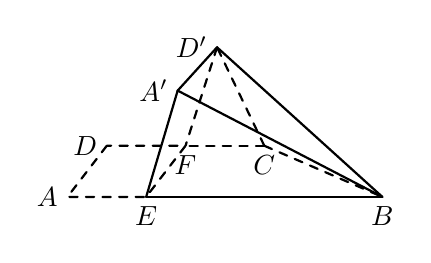
\begin{tikzpicture}[line join=round]
    \tkzDefPoints{0/0/B,-3/0/E,-4/0/A}
    \tkzDefPoints{-1.5/.65/C,-2.5/.65/F,-3.5/.65/D}
    \tkzDefPoints{-2.6/1.35/A',-2.1/1.9/D'}
    \tkzDrawPolygon[dashed,thick](D,A,E,F)
    \tkzDrawSegments[thick](B,E E,A' A',D' D',B A',B)
    \tkzDrawSegments[dashed,thick](C,F C,B C,D' D',F)
    \tkzLabelPoints(E,B,C,F)
    \tkzLabelPoints[left](A,D,A',D')
\end{tikzpicture}

\end{document}
